\chapter{Future Work Plan}
\label{chap:future}

TODO: finalize fields of application
TODO: talk a little bit more in the section on planned papers: first do the studies in the reports and then condense papers out of it as requested
TODO: rework the Gantt-Chart
TODO: rewrite Abstract
TODO: read all again and rework parts which are in strong contrast to the new objectives

major changes
	- as requested, completely reconsidered the aims \& objectives and rewrote the chapter on it which is now much shorter, more concise and scientifically approachable.
	- although not requested, completely rewrote chapter on future work which gives a detailed plan for the research to undertake in the 2nd year, which will focus on the missing "metrication" of my research conducted so far and of the aim in general. the 3rd year research is only outlined in small detail and can still be subject to change.
	- added a section on Fields of Application in the chapter on Reflecting the Literature in which I - also as requested - shortly discuss why the fields of ACE and ABSS were selected as the use-cases in which to conduct the research
	- reworked the Gantt-chart which is much smaller and contains only the mile-stones of the future work chapter
	
minor changes
	- abstract rewritten
	- small changes throughout the text when the content was in to strong contrst to the new objectives

In this chapter we discuss in more detail how we plan to approach the aim and objectives stated in Chapter \ref{chap:aimsObj}. Further we present important milestones, relevant conferences and a Gantt-Chart \ref{fig:gantt} reflecting the most important activities.

\section{Approaching the Objectives}

\subsection{Tools and foundations}
In the first year a prototype of the library should be implemented with a few examples to early gain a good understanding of the topic and to be able to judge whether it is a dead-end or not. This has already successfully happened: the library prototype exists with a number of non-trivial examples including a full implementation of the Sugarscape model. The library is termed FrABS \footnote{Note that - despite it took quite some effort - this library in itself is no the contribution of this Ph.D. but just a means to an end which allows to research and investigate the objectives and research questions and substantiate the hypotheses.} and is described in Appendix \ref{app:frABS}.

To be able to compare our approach to the existing state-of-the-art in the field of ABS we will use the existing library Repast Java. This will allow us to compare the dominant object-oriented paradigm in the field to our approach, discuss similarities and differences and identify draw benefits and drawbacks. 

Clarification on the fundamental challenges in implementing ABS from a programming-paradigm agnostic perspective must be done. This was already conducted in the first paper on Update-Strategies in ABS, which is now accepted at SSC2017 and can be found in Appendix \ref{app:updateStrategies}

\subsection{Pure functional and object-oriented paradigms}
The next objective is then to investigate the fundamental differences between the pure functional and object-oriented paradigms in implementing ABS with their respective incarnations Haskell and Java. This research should be conducted in the form of a report because as it imposes no limits on content-size, is easier to be incorporated in the thesis than a paper and if required a paper can be condensed out of it.
This work should pick up the work of the Update-Strategies paper and broaden and deepen its approach: show in more depth and in more detail which problems need to be solved when implementing an ABS and how both paradigms can be used in their way to solve them and identify potential benefits and drawbacks. There exists already code in Haskell and Java without any additional libraries (except JDK and Haskells standard library called Prelude) produced for the Update-Strategies paper which can be used for this work.
In the next step we need to go up the abstraction ladder and investigate how FrABS and Repast Java approach these problems and compare them from a programing paradigm perspective and identify potential benefits and drawbacks.
As examples the SIR compartment model in epidemiology should be implemented both as a System-Dynamics and ABS 2D-spatial/network model. Also a full implementation of Sugarscape should be attempted in Repast Java \footnote{There exists already an implementation of Chapter II in the Repast Java Demo library upon which we can build.}.
The questions we want to answer in this objective are
\begin{itemize}
	\item What are the approaches of pure functional and object-oriented programming to ABS?
	\item What are the benefits/drawbacks of Haskell and what are the benefits/drawbacks of Java in implementing ABS?
	\item Are the benefits/drawbacks orthogonal to each other e.g. are the weaknesses of one language the other languages strength?
	\item Are there things which are unique when doing Haskell in ABS and cannot be done in a Java approach and vice versa?
\end{itemize}

At least half of the second year will be allocated to this very important research as it lays the very foundations. We conjecture that the conclusion of this research will be that both approaches - paradigms and libraries - though solving specific problems different, are basically equally powerful in implementing the given examples and ABS in general with no fundamental impossibilities on either side. The main noteable (but not fundamental) differences will be performance and memory-consuption, lines-of-code, expressiveness, usability, learning curve and they way to think about ABS.
The question is then: why go through all the pain? Is there a difference? Can't we build somehow on the promised benefits of pure functional programming as in Haskell \footnote{Explicit about side-effects, strong static type-system, algebraic reasoning, declarative style, lambda calculus}?

\subsection{Robustness and correctness}
The answer to the previous question is attempted in a second study, which will look into how pure functional programming can increase robustness, testability, verification and correctness of Agent-Based Simulations. Again the approach will be in writing a report so not to restrict the size of the content, make it easier to incorporate it in the final thesis and condense a paper out of it if required.
Again Repast Java and FrABS Haskell will be used as tools to investigate the research question by investigating the examples implemented in the previous report. The following investigations should be made:

\begin{itemize}
	\item Compare the potential for bugs at runtime e.g. which are not possible to detect at compile time. 
	\item Reproducibility robustness: can unpredictable side-effects affect the systems behaviour? Can such side-effects be guaranteed to not show up? 
	\item Testing and testability of an implementation: how well can we test it using automated tests e.g. unit-tests, property-tests?
	\item Verification of an implementation: can we verify the correctness of a model or at least of parts of the specification?
	\item Can we establish a measure of correctness?
\end{itemize}

The second half of the 2nd year is allocated to this work.

We conjecture that this research will come to the conclusion that pure functional programming dramatically increases the robustness and correctness of an ABS and that it allows for easier and clearer approach to verification using specification testing in QuickCheck and automated testing using Unit- and Property-Testing.

\subsection{Reasoning about dynamics}
This objective investigates how far we can get using the pure functional paradigms ability to reason about a program when applying it to reason about the dynamics of an ABS. As use-cases the idea is to look into reasoning about the equivalence of SD- and ABS-implementation of the SIR compartment model in epidemiology and about the equilibrium dynamics of the bilateral decentralized bartering in Sugarscape.

Both the System-Dynamics and Agent-Based implementation of the SIR compartment model in epidemiology lead to the same dynamics or put different: the Agent-Based implementation shows the same dynamics of the SD implementation when using replications. This is shown by plotting the dynamics as graphs. 

In the Sugarscape model where agents engage in bilateral decentralized bartering Equilibrium is only reached when neo-classical agents are used which don't die of natural age. The equilibrium is not reached when more realistic assumptions are made. This is shown by plotting the prices over time. 

In this part of the Ph.D. we want to answer the following questions:
\begin{itemize}
	\item What and to which extent can we reason about an Agent-Based Simulation in pure functional programming in general and using FrABS in particular?
	\item Can we show that the SD and ABS implementations are equivalent through reasoning about the code?
	\item Can we show that the equilibrium in the decentralized bilateral bartering of Sugarscape is reached / not reached when using neo-classical agents / realistic agents through reasoning about the code?
\end{itemize}

We are very well aware that this topic alone could justify a Ph.D. on its own and it is unsure if we would could make it this far e.g. if the previous research takes longer than anticipated. Still we want to explicitly have clearly stated these objectives and outlined how to approach them - the worst which can happen is that they merely serve as a very in-depth outlook on future research.
Thus the outcome of this research is highly uncertain but the conjecture is that we come to the following conclusion: it highly depends on the complexity and semantics of the model. In the case of the SIR compartment model we expect a success. In the case of the bilateral decentralized bartering in Sugarscape we probably will gain some insights but that at some point due to the interlocking of so many mechanisms it would get too complicated and a full and formal treatment is out of the scope of this Ph.D.
We allocate the first half of the 3rd year to this work.

\section{Thesis}
We leave the following question to be answered in the final thesis:
Do the findings on using the pure functional programming paradigm in ABS apply only to the field of Agent-Based Social Simulation and Agent-Based Computational Economics or to ABS in general?

\section{Planned Papers}
For the remainder of the PhD we planned for two more papers with one targeted as another conference paper and the second one as a journal paper.

\section{Conferences}
\begin{itemize}
	\item \textbf{Multi-Agent Systems AAMS} - General Multi-Agent Systems and Agent-Based Modelling \& Simulation, Deadline in November
	\item \textbf{Social Simulation Conference SSC} - New Methods and models in simulation, Deadline in March
	\item \textbf{Symposium on Trends in Functional Programming} - Functional programming stuff, Deadline in May
\end{itemize}

\section{Mile-Stones}
\begin{itemize}
	\item 2017 31st March - finished and submit 1st paper 
	\item 2017 21st July - 1st annual review
	\item 2017 October - 2nd year starts, investigate programming paradigms
	\item 2017 Februaray - finished programming paradigms, start robustness and correctness
	\item 2017 September - finished robustness and correctness
	\item 2018 October - 3rd year starts, investigate reasoning
	\item 2018 March - finished reasoning
	\item 2019 April - Begining of thesis-writing
	\item 2019 September - Submit thesis
	\item 2019 30th September - official end of PhD
	\item 2020 30th September - end of pending-period
\end{itemize}

\label{app:gantt}
\begin{landscape}
	\begin{figure}
		\label{fig:gantt}
  		\caption{Gantt-Chart for remaining PhD}
  		\centering
  		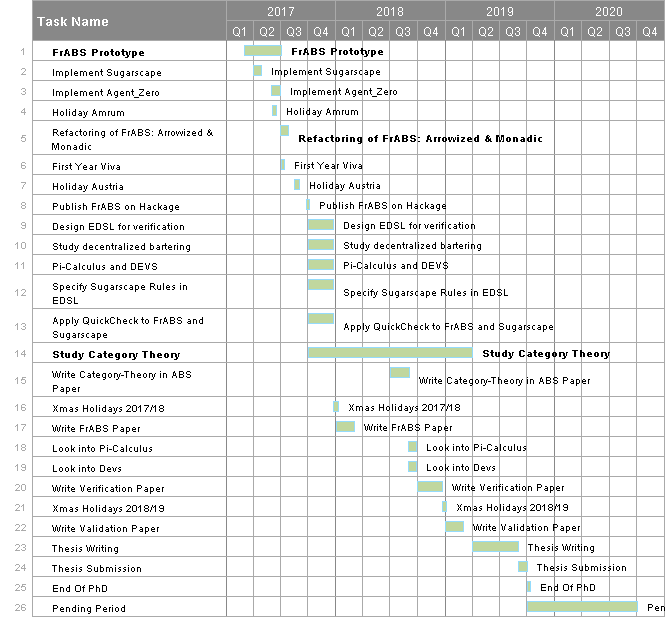
\includegraphics[width=1.2\textwidth]{./charts/gantt.png}
	\end{figure}
\end{landscape}